%% Proposed replacement for \subsection{Acceptance} in sec/section4_nosat.tex.
%% Keeps the label ss:loop and the labels M1, M2; adds def:children, def:graph.
%% 
% \rlink expands to bare math; \rl is the text-mode-safe form used below.
\newcommand{\rl}[1]{\ensuremath{\rlink{#1}}}

\subsection{Two Worked Runs of The Tableau}\label{ss:ex}


Consider the formula $\mathrm{AG}\,\mu\wedge\mathrm{AG}(q\rightarrow\sigma)$ with $\mu=\tAU{\top}{q}{[1,4]}$, that is $\mathrm{AF}_{[1,4]}q$, and 
$\sigma=\tAR{\bot}{\neg q}{(0,3]}$, that is $\mathrm{AG}_{(0,3]}(\lnot q)$. The first conjunct demands a $q$ within
$[1,4]$ of every configuration; the second forbids a $q$ for $3$ time units after each one. The left conjunct proceeds as a persistent demand. Its first demand launches $\mu^\bullet$ with $x$
reset and the deadline $x\le\sup\kI=4$; the next re-demand meets a live pursuit, so \ruleref{Carry}
folds it in and the pursuit becomes $\mu^{\ast}$. Meanwhile the right conjunct re-imposes its body
$\neg q\vee\sigma$ at every configuration, so $N_2$ carries both, and the disjunction is settled
before $\mu^{\ast}$ is unfolded.
\noindent
Take $\neg q$, at $N_3$. The pursuit can then neither take \ruleref{Ustopcarry} nor \ruleref{Ugocarry}: \ruleref{Ustopcarry} would assert
$q$ into a goal set already holding $\neg q$, and \ruleref{Ugocarry} can only defer, which past $x=4$
empties the zone against the deadline. Both children close.
\noindent
Take $\sigma$ instead. It is launched with its own clock $z$ reset, and \ruleref{Ustopcarry} asserts
$q$, re-zeroing $x$ and recapping it at $b-a=3$; this is $N_4$, where the two clocks begin to run
together, $x=z$. That is the contradiction. The carried deadline $x\le3$ says the next $q$ is due
within $3$, while $\sigma$ forbids $q$ for as long as $z\in(0,3]$. At $N_5$ the \ruleref{Ustopcarry} branch needs a
$q$ it cannot have, and \ruleref{Ugocarry} needs $x>3$, which the deadline denies. Both children close,
so $N_2$ closes and the formula is \UNSAT.


\begin{figure}[h]
\centering
\begin{subfigure}[b]{0.5\textwidth}\centering
\resizebox{0.8\linewidth}{!}{%
\begin{tikzpicture}[
  every node/.style={align=center, font=\scriptsize},
  level 1/.style={sibling distance=26mm, level distance=9mm},
  level 2/.style={sibling distance=30mm, level distance=11mm},
  level 3/.style={sibling distance=15mm, level distance=11mm},
  level 4/.style={sibling distance=15mm, level distance=11mm},
  edge from parent/.style={draw,-}
]
\node {$N_0:\{\mathrm{AG}\,\mu\wedge\mathrm{AG}(q\!\rightarrow\!\sigma)\}\ \ANDn$}
 child { node {$N_1:\{\,\}$\\ $\OPEN$}
   edge from parent node[left,font=\tiny,pos=.45]{\rl{discharge}} }
 child { node {$N_2:\{\mu^{\ast},\neg q\vee\sigma\},\ x{:=}0$\\ $\Deadline{=}\{x\le 4\}\ \ORn$}
   child { node {$N_3:\{\neg q,\mu^{\ast}\}\ \ORn$}
     child { node {$\CLOSED$\\ $q\wedge\neg q$}
       edge from parent node[left,font=\tiny,pos=.45]{\rl{Ustopcarry}} }
     child { node {$\CLOSED$\\ $\rl{Ugocarry}$\\ needs $x>4$}
       edge from parent node[right,font=\tiny,pos=.45]{\rl{Ugocarry}} }
     edge from parent node[left,font=\tiny,pos=.45]{$\neg q$} }
  child { node {$N_4:\{q,\mu^{\ast},\sigma^\bullet\}$\\ $x{:=}0,\ z{:=}0,\ \Deadline{=}\{x\le3\}$}
     child { node {$N_5:\{\neg q,\mu^{\ast},\sigma^\bullet\}$\\ $x{=}z\in(0,3]\ \ORn$}
       child { node {$\CLOSED$\\ \rl{Ustopcarry} \\needs $q$}
         edge from parent node[left,font=\tiny,pos=.45]{\rl{Ustopcarry}} }
       child { node {$\CLOSED$\\ \rl{Ugocarry} \\needs $x>3$}
         edge from parent node[right,font=\tiny,pos=.45]{\rl{Ugocarry}} }
       edge from parent node[right,font=\tiny,pos=.45]{\rl{Delay}, \rl{EX}} }
     edge from parent node[right,font=\tiny,pos=.4]{$\sigma$; \rl{launch}, \rl{Ustopcarry}} }
   edge from parent node[right,font=\tiny,pos=.45]{$(\wedge)$, \rl{launch}, \rl{Carry}} };
\end{tikzpicture}}
\subcaption{$\mathrm{AG}(\mathrm{AF}_{[1,4]} q)\wedge\mathrm{AG}(q \rightarrow
\mathrm{AG}_{(0,3]}(\lnot q))$.}
\label{fig:ex-roll}
\end{subfigure}
\hfill
\begin{subfigure}[b]{0.48\textwidth}\centering
\resizebox{0.9\linewidth}{!}{%
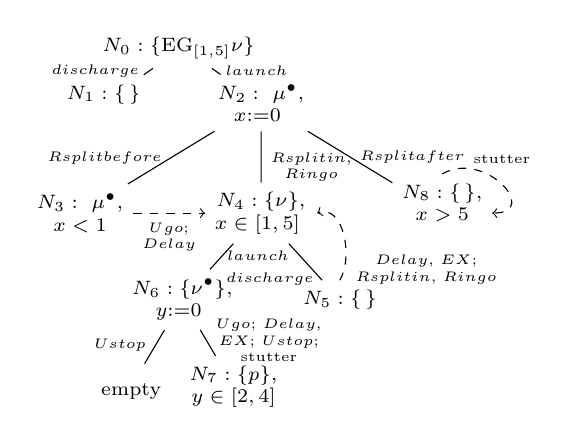
\begin{tikzpicture}[
  every node/.style={align=center, font=\scriptsize},
  level 1/.style={sibling distance=20mm, level distance=7mm},
  level 2/.style={sibling distance=23mm, level distance=14mm},
  level 3/.style={sibling distance=20mm, level distance=11mm},
  level 4/.style={sibling distance=13mm,level distance=11mm},
  edge from parent/.style={draw,-}
]
\node {$N_0:\{\mathrm{EG}_{[1,5]}\nu\}\ \ANDn$}
 child { node {$N_1:\{\,\}$\\ $\OPEN$}
   edge from parent node[left,font=\tiny,pos=.45]{\rl{discharge}} }
 child { node {$N_2:\ \mu^\bullet,$\\$x{:=}0\ \ANDn$}
   child { node (bef) {$N_3:\ \mu^\bullet,$\\$ x<1$}
    edge from parent node[left,font=\tiny,pos=.5]{\rl{Rsplitbefore}} }
   child { node (in) {$N_4:\{\nu\},$\\$ x\in[1,5]\ \ANDn$}
     child { node {$N_6:\{\nu^\bullet\},$\\$ y{:=}0\ \ORn$}
       child { node {$\CLOSED$\\ empty}
         edge from parent node[left,font=\tiny,pos=.45]{\rl{Ustop}} }
       child { node {$N_7:\{p\},$\\$ y\in[2,4]$}
         edge from parent node[right,font=\tiny,pos=.4]{\rl{Ugo}; \rl{Delay},\\ \rl{EX}; \rl{Ustop}; \\stutter} }
       edge from parent node[right,,xshift=-2pt,font=\tiny,pos=.45]{\rl{launch}} }
       child { node (disch) {$N_5:\{\,\}$}
       edge from parent node[left, yshift=-7pt,xshift=7pt,font=\tiny,pos=.45]{\rl{discharge}} }
     edge from parent node[right,font=\tiny,pos=.7]{\rl{Rsplitin},\\ \rl{Ringo}} }
   child { node (aft) {$N_8:\{\,\},$\\$ x>5$\\ $\OPEN$}
     edge from parent node[right,font=\tiny,pos=.5]{\rl{Rsplitafter}} }
   edge from parent node[right,font=\tiny,pos=.45]{\rl{launch}} };
\draw[->,dashed] (bef.east) to[out=0,in=180,looseness=.7]
  node[below,font=\tiny,pos=.5]{\rl{Ugo}; \\\rl{Delay}} (in.west);
\draw[->,dashed] (disch.north) to[out=60,in=20,looseness=1]
  node[right,yshift=-4pt,font=\tiny,pos=.25]{\rl{Delay}, \rl{EX};\\ \rl{Rsplitin}, \rl{Ringo} } (in.east);



\draw[->,dashed] (aft.north) to[out=30,in=0,looseness=2]
  node[above, yshift=4pt,font=\tiny]{stutter} (aft.east);
\end{tikzpicture}}
\subcaption{$\mathrm{EG}_{[1,5]}\tEU{\top}{p}{[2,4]}$.}\label{fig:ex-zeno}
\end{subfigure}
\caption{Two tableau runs. %$\ANDn$ marks an AND-node;$\ORn$ an OR-node. 
$\OPEN$ marks an open node, $\CLOSED$ a closed
one.}\label{fig:ex2}
\end{figure}

%\begin{example}%[A Zeno cycle that may be left]\label{ex:zeno}
Consider $\mathrm{EG}_{[1,5]}\,\nu$, where $\nu=\tEU{\top}{p}{[2,4]}$. Write $x$ for the clock of
the release, and $y$ for that of $\nu$. \ruleref{Cov} splits $N_0$ into a discharge child, which
carries no pursuit, and the launch $N_2$, where $x$ is reset. \ruleref{Rsplit} then partitions the zone,
conjunctively, into its three parts. At $N_3$, the \ruleref{Rsplitbefore} part, \ruleref{Delay} carries $x$ into  \kI. $N_8$, where $x>5$, drops $\mu^\bullet$ and leaves a goal-free node that
may delay indefinitely: a time-progressing loop, since no until needs to be fulfilled and $x$ is
extrapolated above $M$.
\noindent
$N_4$ represents the \ruleref{Rsplitin} part of \ruleref{Rsplit}, where $\nu$ is inserted into $\Gamma$ and so
demanded. \ruleref{Cov} applies, giving two conjunctive branches. The \ruleref{launch} child $N_6$
proves $\nu$. It carries $\nu^\bullet$ with $y$ reset; its \ruleref{Ustop} is empty there, the window
$[2,4]$ not yet open, so only \ruleref{Ugo} survives until a delay carries $y$ into $[2,4]$, where
\ruleref{Ustop} asserts $p$ and drops $\nu^\bullet$. The \ruleref{discharge} child $N_5$ drops $\nu$
from $\Gamma$ and carries $\mu^\bullet$ on; a delay and \ruleref{EX} revive the release, still inside
$[1,5]$, and its in-part demands $\nu$ once more. The search is back at $N_4$, closing a loop. That
loop is not time-progressing: $x$ is never reset, and the in-window zone holds it below $5$.
\noindent
Nonetheless, we can construct a successful marking  as $\mathcal M=\{N_0,\allowbreak N_1,\allowbreak N_2,\allowbreak N_3,\allowbreak N_4,\allowbreak N_5,\allowbreak N_6,\allowbreak N_7,\allowbreak N_8\}$. \ref{M2} holds because the only until pursuit is $\nu^\bullet$, active at $N_6$, and the path to
$N_7$ takes its \ruleref{Ustop} at a node whose zone meets $y\in[2,4]$. \ref{M1} holds because every node of
$\mathcal M$ reaches a time-progressing loop: the nodes carrying the release reach $N_8$ by delaying
until $x$ passes $5$, which lapses it, while $N_1$ and, once $\nu^\bullet$ is dropped, $N_7$ carry
no pursuit, so no deadline caps their delays and their stutter loops are time-progressing. So $\mathcal M$, as well as the tableau, are successful and
$\mathrm{EG}_{[1,5]}\,\nu$ is \SAT.
 still follows it.

\subsection{The Tableau Graph and Acceptance}\label{ss:loop}

Through application of the rules, the tableau builds a graph of nodes, which can be used to establish satisfiability. 




To build this graph we settle which rule fires at a node, since rule application is
non-deterministic: several rules may apply to a node, which inherits the kind of the rule fired at it, and
one rule may apply to several goals.
Writing $\Subt(\varphi)$ for the timed modalities of $\FL(\varphi)$ and
$P=\FL(\varphi)\cup\{\mu^\bullet,\mu^{\ast}\mid\mu\in\Subt(\varphi)\}$, we define
$\FL^{\bullet}(\varphi)=P\cup\{\EX\chi,\AX\chi\mid\chi\in P\}$, with $|\FL^{\bullet}(\varphi)|=O(|\FL(\varphi)|)$. No rule produces a goal or a
context formula outside $\FL^{\bullet}(\varphi)$.



We fix, arbitrarily, a linear order \FormalSmaller{} on formulas (e.g., lexicographic)
and fire on the \FormalSmaller-least goal of $\Gamma$ to which a rule applies: a conjunction \ruleref{Conj}, a disjunction \ruleref{Disj}, an
$\AX\varphi$ \ruleref{AX}, a demanded modality \ruleref{Cov}, \ruleref{Carry} or \ruleref{Absorb}
as their side conditions prescribe, an until pursuit past a bounded window \ruleref{Umiss}, an
ordinary until pursuit $\mu^\bullet$ \ruleref{Uunf}
and a persistent one $\mu^{\ast}$ \ruleref{Uunfcarry}, and a release pursuit
\ruleref{Runf} when its zone lies wholly before or wholly inside
the window and \ruleref{Rsplit} otherwise.

This strategy produces for each node $N$ a set of children $\ch(N)$. A closed node has no children,
and the children of a saturated one are the \ruleref{Delay}- and the
\ruleref{EX}-children together, both successor rules being conjunctive, so it is an \ANDn-node.





The tableau graph $\TabGraph = (\TabNode, \TabEdge)$ is then constructed from the nodes reachable under $\ch$ from the
root $N_0=\tup{\{\varphi\}}{\emptyset}{\{\mathbf 0\}}{\emptyset}{\emptyset}$: its vertices $V$ are
those nodes up to $\equiv$, and it has an edge $e\in E$ from $N$ to every $N'\in\ch(N)$. A \emph{path} of $\TabGraph$ is a sequence of vertices, each a child of the preceding one, and a \emph{cycle} is a path returning to its first vertex.


\begin{lemma}%[Finiteness]
  \label{lem:finiteness}
$|\TabNode|\le 2^{O(n)}\cdot M^{O(n^{2})}$, and every node has $O(n)$ children.
\end{lemma}
\begin{proof}
  Each component of a node ranges over a set of size $2^{O(n)}$: $\Gamma$ and $\Ctx$ over subsets
of $\FL^{\bullet}(\varphi)$; $\obligations$ over subsets of $\Subt(\varphi)$, being determined by
its domain; $\Deadline$ over the assignments to each $x_\mu$ of $\sup\kI$ or $\sup\kI-\inf\kI$ with a
strictness flag; the reset set over subsets of $\clockSet$; and the discharged modality over
$\Subt(\varphi)$. A $\cong_M$-zone over $K\le n+1$ clocks is a $(K{+}1)^{2}$ DBM whose
entries are $\infty$ or lie in $\{-M,\dots,M\}\times\{<,\le\}$, so there are $M^{O(n^{2})}$ of
them. Thus the bound is $2^{O(n)}\cdot M^{O(n^{2})}$. Every rule has at most three children except
\ruleref{EX}, with one per $\EX\psi\in\Gamma$ and $|\Gamma|=O(n)$,.
\end{proof}


A \emph{marking} $\mathcal M \subseteq \TabNode$ is a set of vertices containing no closed node and containing, of each
of its members, at least one child if that node is an \ORn-node and all of them if it is an
\ANDn-node. A cycle of $\mathcal M$ is \emph{time-progressing} if it elapses positive time and every
clock is either reset on it or extrapolated above $M$. 

$\mathcal M$ is \emph{successful} if
every $N\in\mathcal M$ satisfies
\begin{enumerate*}[label={\textbf{(M\arabic*)}}, ref={\textbf{(M\arabic*)}},
                   itemjoin={{; }}, itemjoin*={{; and }}]
\item\label{M1} some path of $\mathcal M$ from $N$ meets a time-progressing cycle
\item\label{M2} for every until pursuit $\mu$ active at $N$,  some path of
$\mathcal M$ from $N$ that carries it throughout, with $x_\mu$ unreset along the way, takes a stop
branch (\ruleref{Ustop} or
\ruleref{Ustopcarry}) at a node $N_k$ with $Z_k\cap(x_\mu\in\kI)\neq\emptyset$.
\end{enumerate*}
\noindent
A tableau \emph{succeeds} on $\varphi$ if $N_0$ lies in a successful marking.


\ref{M2} ensures that an until pursuit is fulfilled rather
than deferred for ever through \ruleref{Ugo}. Its clause on $x_\mu$ ties the stop to the onset
the pursuit measures: a relaunch on the way restarts the clock, and a stop taken past it
witnesses the later onset.
\ref{M1} excludes Zeno witnesses. A clock never reset on a cycle and bounded there by some $k\le M$
caps the delays of all its traversals at $k$, so infinitely many traversals elapse only finitely much
time. The run they describe lies outside $\mathrm{Runs}^\infty$, on which satisfaction is defined,
and is a behaviour no system exhibits. The requirement that a cycle elapse positive time rules out
cycles built from expansion steps alone. Consider a persistent pursuit that has already carried over once: $\psi$ is a goal,
$x_\mu=0$, and the deadline on $x_\mu$ is $b-a$. If $0\in\kI$, a second application of
\ruleref{Ustopcarry} yields the same node, since the goal it adds is already present, the clock
it resets is already zero, and the deadline it sets is already in force. The node is its own
child, and the resulting self-loop elapses no time, so \ref{M1} keeps the node only if another
path leaves it.




%Both clauses read edges and not nodes: \ref{M1} inspects the clocks a cycle resets, \ref{M2} the
%branch on which a pursuit stops. This is why Definition~\ref{def:graph} compares the two records a
%node keeps of them. Without them a node reached through a reset and one reached without it would be
%merged, and a cycle through the merged node could report a reset that it never performs.
%

%
%Not every cycle of $\TabGraph$ crosses a successor step. \ruleref{Ustopcarry} re-imposes $\mu^{\ast}$
%on a node whose zone it has just reset, and for $\inf\kI=0$ the result can be the node it started
%from; Definition~\ref{def:graph} identifies the two, so a chain of rule applications that would
%regress for ever closes a cycle instead. Such a cycle elapses no time, so \ref{M1} discards it, and
%the calculus needs no separate argument that rule application terminates.
%
%Both clauses ask for reachability inside $\mathcal M$ rather than constraining every cycle
%separately, which is what the semantics calls for: TCTL quantifies over time-divergent runs, so what
%a witness owes at a reachable configuration is \emph{one} divergent continuation, not that every
%continuation diverge. Example~\ref{ex:zeno} exhibits a node whose only local cycle is Zeno and which
%belongs to a successful marking nonetheless.
%